\documentclass[10pt, a4paper]{article}
\usepackage[utf8]{inputenc}
\usepackage[paper=a4paper, left=3.0cm, right=3.0cm, bottom=1.5cm, top=3.5cm]{geometry}
\usepackage{mathtools}
\usepackage{float}
%\usepackage{graphicx}
\usepackage[]{algorithm2e}
\usepackage{amssymb}
\usepackage{subcaption}

\usepackage[conEntregas]{caratula}

\begin{document}

\titulo{Trabajo Pr\'actico 1}

\fecha{10/04/2015}

\materia{Introducción al Procesamiento Digital de Imágenes}

\integrante{Dellanzo, Claudia Antonella}{019/13}{antodellanzo@gmail.com}
\integrante{Julián Bayardo}{850/13}{julian@bayardo.info}
% Pongan cuantos integrantes quieran

\maketitle
\tableofcontents

\newpage

\section{Introducción}

El objetivo de este trabajo prático es implementar un algoritmo para realzar imágenes a través de la ecualización de histogramas siguiendo lo propuesto en el paper \textit{Adaptive extended piecewise histogram equalisation for dark image enhancement} \cite{paper}. Aparte de esto, se buscará realizar un estudio sobre la selección de parámetros (en cuántos histogramas partir el original y la selección de $\alpha$ y  $\beta$).

\section{Implementación}

Para la implementación del algoritmo seguimos el propuesto en el paper, el cual es:

\begin{figure}[H]
	\centering
    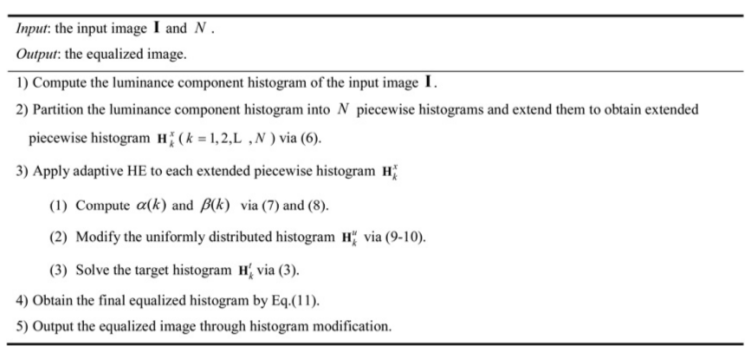
\includegraphics[width=\textwidth]{algoPaper.png}
    \caption{Algoritmo propuesto}
\end{figure}

El método llamado \textbf{AEPHE} toma como parámetro obligatorio de entrada la imagen y le aplica todas las transformaciones propuestas. Aparte, hay otros parámetros de entrada opcionales:
\begin{itemize}
\item \textit{Alphas:} Toma un vector de $\alpha$'s, los cuales serán aplicados en orden a cada subhistograma generado durante el algoritmo.
\item \textit{Betas:}  Toma un vector de $\beta$'s, los cuales serán aplicados en orden a cada subhistograma generado durante el algoritmo.
\item \textit{Gammas:} Toma un vector de $\gamma$'s, los cuales serán aplicados en orden a cada subhistograma generado durante el algoritmo.
\item \textit{number\textunderscore of\textunderscore histogramas:} Cantidad de histogramas en los que se desea partir el histograma original de la imagen de entrada. El valor es $3$ por defecto.
\item \textit{discretization\textunderscore bin\textunderscore width:} Cantidad de \textit{bins} en los que se dividirá el histograma al momento de realizar la conversión para trabajar con enteros o floats. El valor es $1/255$ (255 bins) por defecto. 
\item \textit{plot\textunderscore intermediate\textunderscore histograms:} Booleano que indica si se quiere ir mostrando las figuras de todos los subhitogramas generados durante la ejecución del algoritmo. El valor es \textit{False} por defecto.
\end{itemize}

La razón por la cual tomamos vectores de valores en algunos parámetros será explicada posteriormente cuando hablemos sobre la experimentación y los problemas con los que nos encontramos al realizar los mismos.

Si el vector de $\gamma$'s no se especifica, tomamos todos los valores como 0 ya que dicho parámetro no contribuye notablemente al realce de la imagen. Si alguno de los otro dos vectores (vector de $\alpha$'s o $\beta$'s) es nulo, luego se procede a calcularlos de la manera que lo indica el paper:

\begin{equation}
\alpha = \dfrac{M_{i}}{M_{i} + M_{c}}
\end{equation}
\begin{equation}
\beta = \dfrac{M_{c}}{M_{i} + M_{c}}
\end{equation}

\begin{figure}[H]
	\centering
    \begin{subfigure}{0.5\textwidth}
        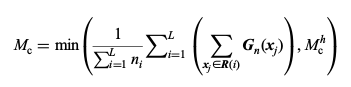
\includegraphics[width=0.9\textwidth]{calculo-Mc.png}
    \end{subfigure}\hfill
    \begin{subfigure}{0.5\textwidth}
        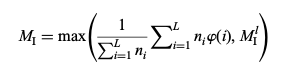
\includegraphics[width=0.9\textwidth]{calculo_Mi.png}
    \end{subfigure}\hfill
\end{figure}

Cada uno de estos valores se calcula para cada subhistograma generado.

\section{Experimentación}

\subsection{Experimentando con imágenes tanto claras como oscuras}

Para los siguientes experimentos utilizamos fotos tomadas por nosotros de día cuya característica es que poseen partes muy claras y otras muy oscuras. La idea era observar cómo se comporta nuestro algoritmo seleccionando los valores de $\alpha$ y $\beta$ de manera automática, y tomando valores de $\gamma = 0$ y $k=3$. 

\subsubsection{Experimento 1}

Para realizar este experimento seleccionamos imágenes tomadas a contra luz para ver cómo afectaba la presencia del sol en la misma. Al comienzo de este experimento, utilizabamos siempre un único valor de $\alpha$ y $\beta$. Estos valores  nos sirven para decidir cuánto peso darle al histograma uniforme y  original, lo cual se deduce de la fórmula:

\begin{figure}[H]
	\centering
        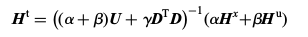
\includegraphics[width=0.5\textwidth]{calculo-H.png}
\end{figure}

Obteníamos secciones de la imagen que en la original eran muy claras y en la ecualizada final quedaban completamente negras:

\begin{figure}[H]	
	\centering
    \begin{subfigure}{0.5\textwidth}
	\centering
        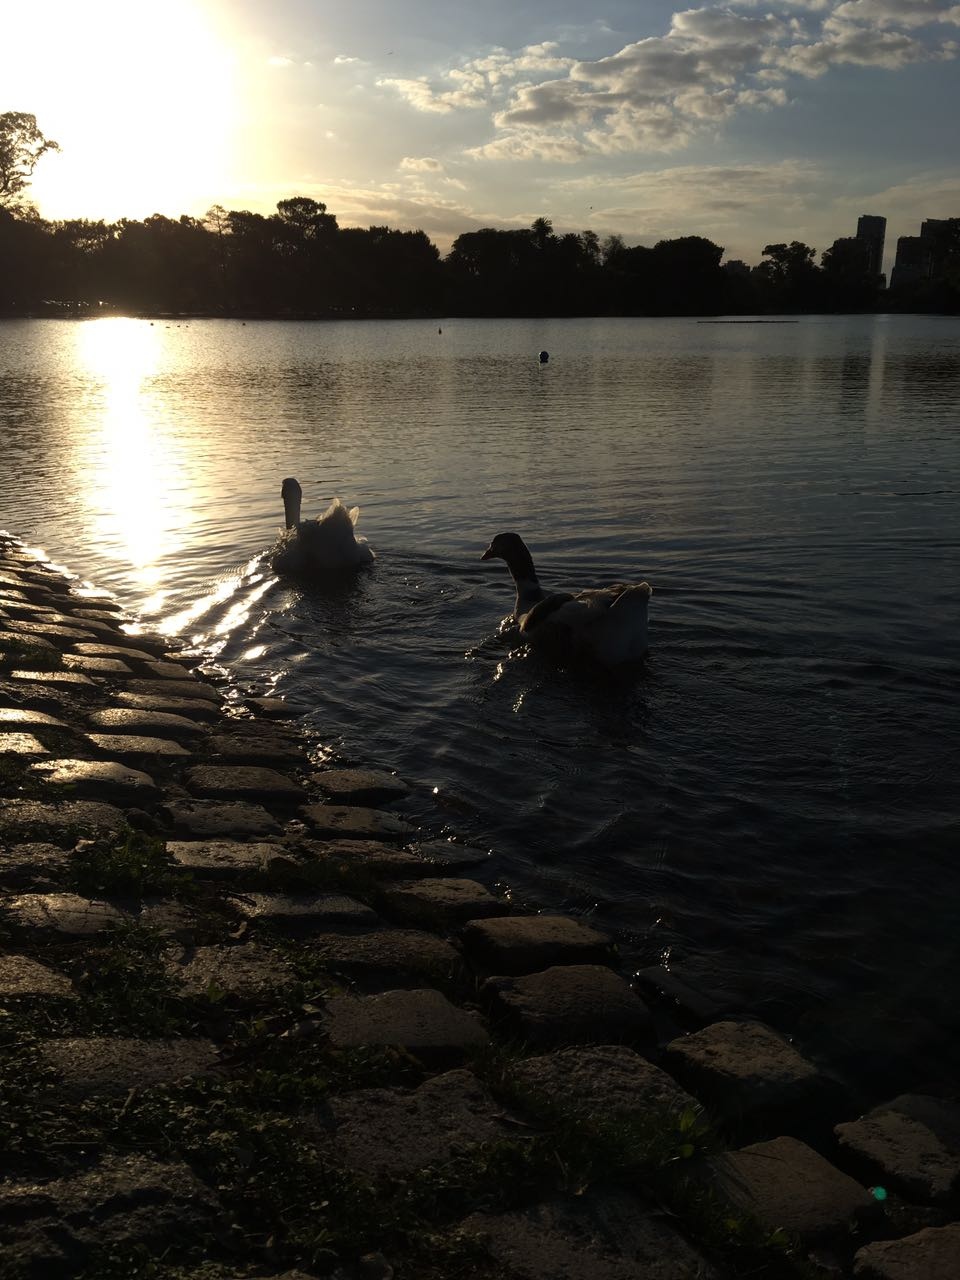
\includegraphics[width=0.9\textwidth]{patitos1.jpg}
        \subcaption{Imagen original}
    \end{subfigure}\hfill
    \begin{subfigure}{0.5\textwidth}
    	\centering
        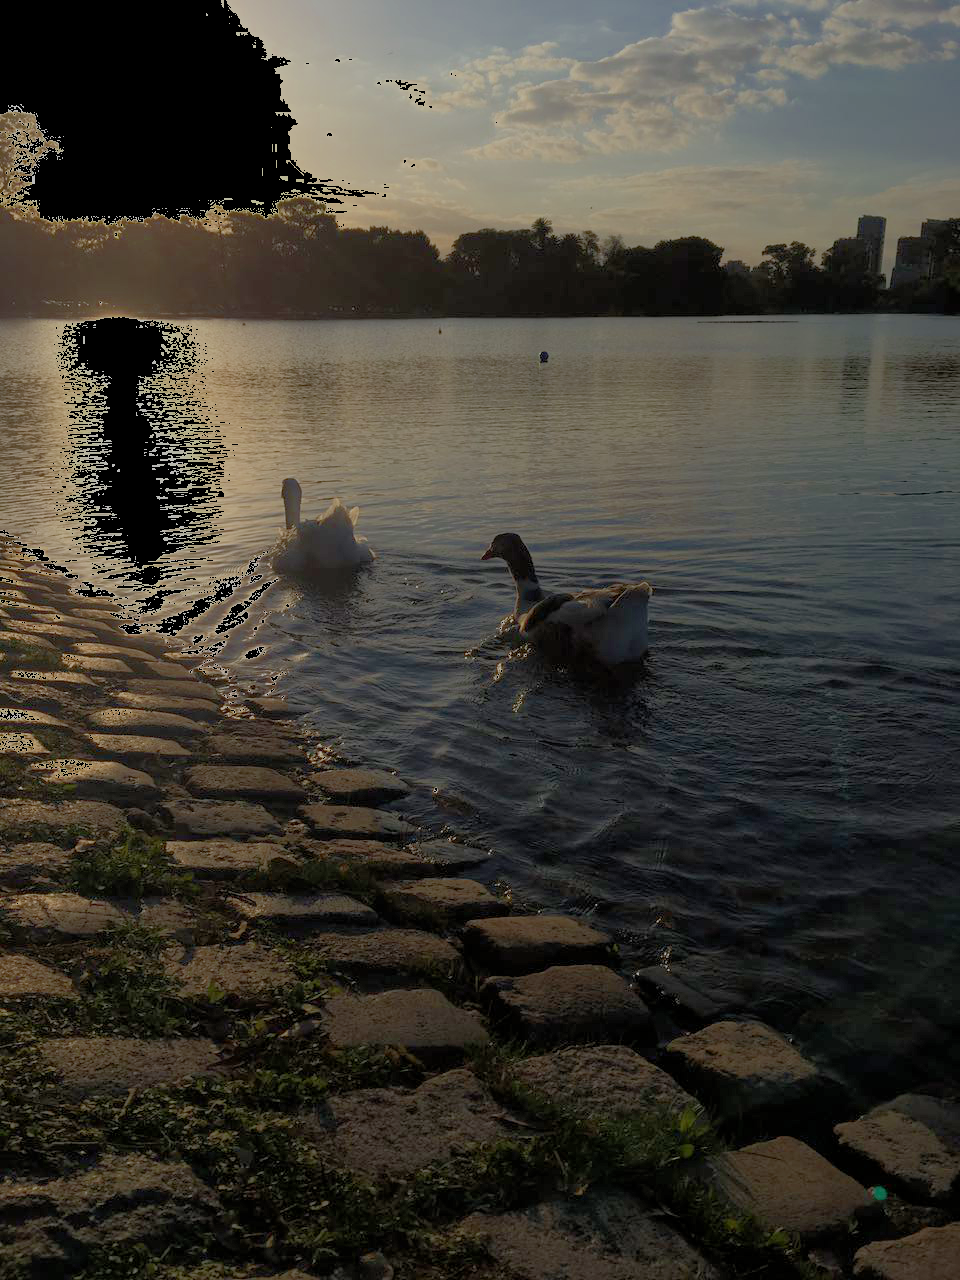
\includegraphics[width=0.9\textwidth]{patitos1_ecualizada.png}
        \subcaption{Imagen luego de ser ecualizada}
    \end{subfigure}\hfill	
\end{figure}

Así, encontramos que dado que la imagen posee partes muy claras, hay un problema al momento de ecualizar aquellas secciones. Por esta razón, decidimos que nuestro algoritmo tome un vector de valores de $\alpha$'s y $\beta$'s, para poder decidir en cada subhistograma si darle más peso al original o al uniforme. 
Luego, procedimos a seleccionar valores específicos para dichos parámetros de forma tal que nuestra imagen sea  correctamente ecualizada. Por ejemplo, variando los parámetros de la imagen anterior obtuvimos el siguiente resultado:

\begin{figure}[H]	
	\centering
    \begin{subfigure}{0.5\textwidth}
	\centering
        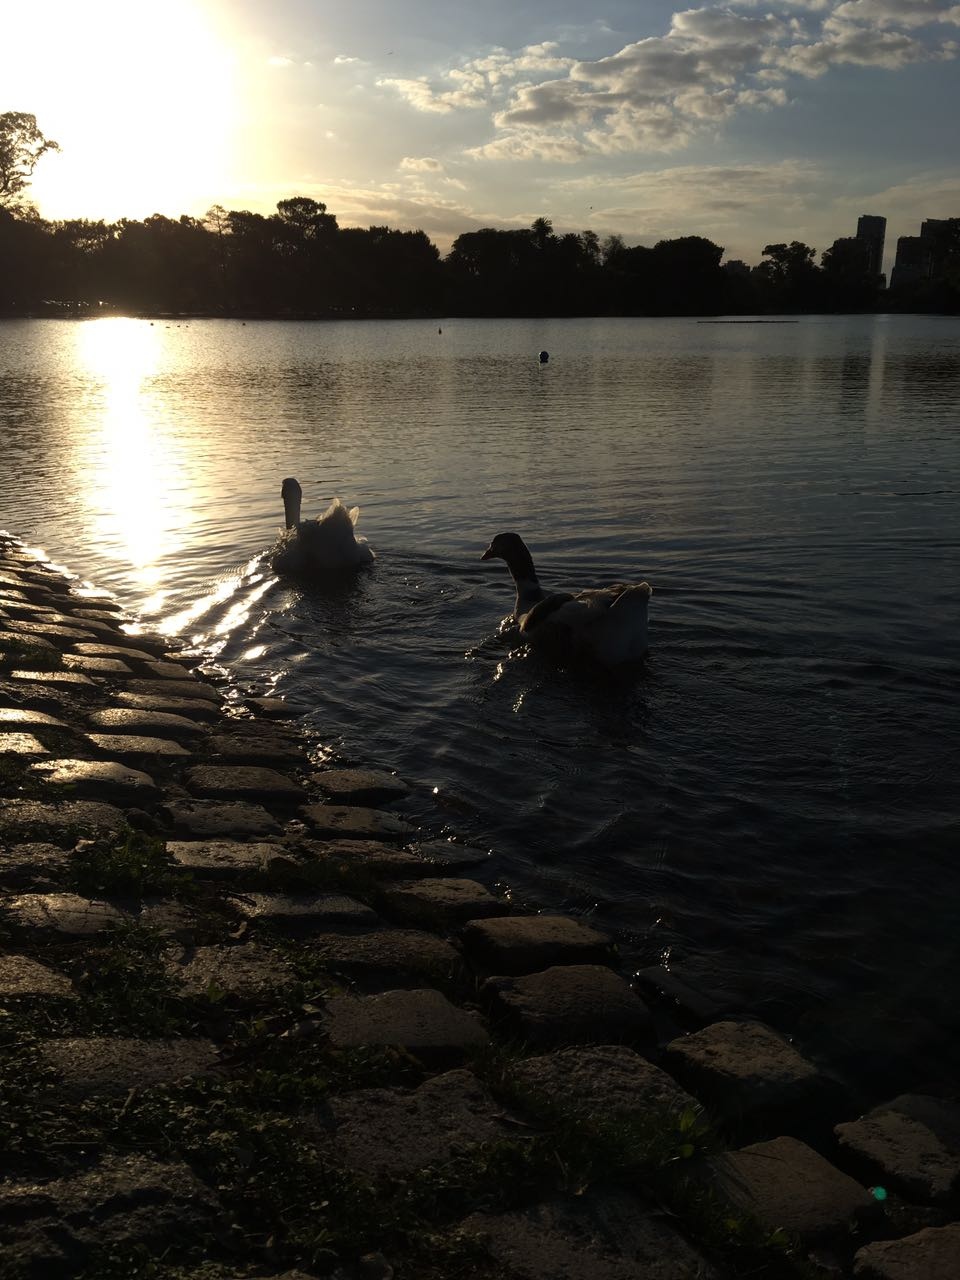
\includegraphics[width=0.5\textwidth]{patitos1.jpg}
        \subcaption{Imagen original}
    \end{subfigure}\hfill
    \begin{subfigure}{0.5\textwidth}
    	\centering
        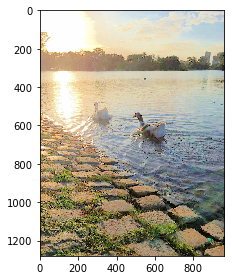
\includegraphics[width=0.63\textwidth]{patitosclaro.png}
        \subcaption{Imagen luego de ser ecualizada con $k=3, \alpha = [1, 1, 0], \beta = [0, 0, 1]$}
    \end{subfigure}\hfill	
\end{figure}

\subsubsection{Experimento 2}

En este experimento utilizamos unas imágenes tomadas mientras anochecía, en la cuales todavía había rastros de luz en el cielo. Éstas tienen la particularidad de ser tanto muy oscuras como muy claras. Al ejecutar nuestro algoritmo, ya trabajando con vectores automatizados de parámetros, obtuvimos problemas similares que con el experimento anterior, en los que el cielo se pintaba de negro:

\begin{figure}[H]	
	\centering
    \begin{subfigure}{0.5\textwidth}
	\centering
        \includegraphics[width=0.9\textwidth]{rosedal_original.png}
        \subcaption{Imagen original}
    \end{subfigure}\hfill
    \begin{subfigure}{0.5\textwidth}
    	\centering
        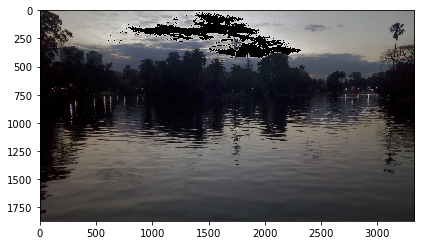
\includegraphics[width=0.9\textwidth]{rosedal-algoritmo.png}
        \subcaption{Imagen luego de ser ecualizada}
    \end{subfigure}\hfill	
\end{figure}

\begin{figure}[H]	
	\centering
    \begin{subfigure}{0.5\textwidth}
	\centering
        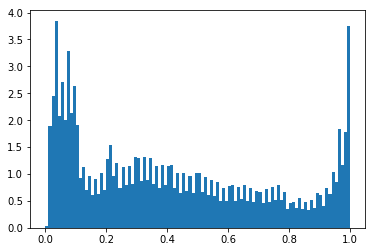
\includegraphics[width=0.9\textwidth]{rosedal-histograma-original.png}
        \subcaption{Histograma de imagen original}
    \end{subfigure}\hfill
    \begin{subfigure}{0.5\textwidth}
    	\centering
        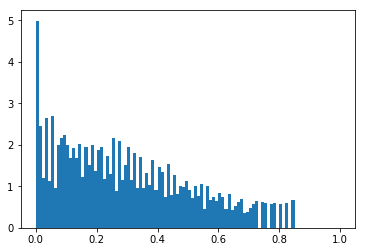
\includegraphics[width=0.9\textwidth]{rosedal-histograma-final.png}
        \subcaption{Histograma ecualizado final}
    \end{subfigure}\hfill	
\end{figure}

Al ir viendo los valores de $\alpha$ y $\beta$ que nuestro algoritmo generaba, veíamos que tomaba valores muy altos de $\beta$, dándole muy poco peso a la imagen original. Por esto decidimos modificar la cota inferior de $M_{I}$ ($M_{I}^l$) utilizada al momento de calcular el $\alpha$ y $\beta$ automatizado, para exigirle que mantenga parte de la imagen original siempre y no le asigne tanto peso al histograma uniforme, obtuviendo el siguiente resultado:

\begin{figure}[H]	
	\centering
    \begin{subfigure}{0.5\textwidth}
	\centering
        \includegraphics[width=0.9\textwidth]{rosedal_original.png}
        \subcaption{Imagen original}
    \end{subfigure}\hfill
    \begin{subfigure}{0.5\textwidth}
    	\centering
        \includegraphics[width=0.9\textwidth]{rosedal_ecualizada.png}
        \subcaption{Imagen luego de ser ecualizada}
    \end{subfigure}\hfill	
\end{figure}

Acá se puede observar que la imagen, si bien no quedó con secciones negras, se oscureció en vez de aclararse.  Por esta razón decidimos que para imágenes con características como estas, seleccionar automatizadamente los valores de los parámetros no nos estaba resultando, por lo que recurrimos a seleccionarlos nosotros mismos para intentar ecualizar correctamente la imagen. Obtuvimos el siguiente resultado:

\begin{figure}[H]	
	\centering
    \begin{subfigure}{0.5\textwidth}
	\centering
        \includegraphics[width=0.7\textwidth]{rosedal_original.png}
        \subcaption{Imagen original}
    \end{subfigure}\hfill
    \begin{subfigure}{0.5\textwidth}
    	\centering
        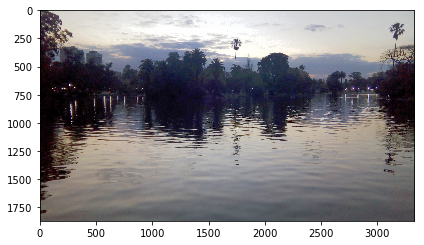
\includegraphics[width=0.8\textwidth]{rosedal-101-010.png}
        \subcaption{Imagen luego de ser ecualizada con $k=3, \alpha = [1, 0, 1], \beta = [0, 1, 0]$}
    \end{subfigure}\hfill	
\end{figure}

\subsection{Experimentos con imágenes oscuras}

Para este experimento observamos el comportamiento de nuestro algoritmo sobre imágenes oscuras, varias de ellas provistas por la cátedra. Utilizamos el cálculo automatizado de valores de $\alpha$ y $\beta$, con $\gamma = 0$ y $k=3$.

Al observar estos problemas, decidimos modificar el valor de $M_{I}^l$ para mantener parte de la imagen original y no provocar una sobre\-ecualización de la imagen. Por ejemplo, tomando $M_{I}^l=0.8$, obtuvimos los siguientes resultados:



\subsection{Variación de parámetros}

Para esta parte buscamos experimentar variar el valor de K, el cual indica la cantidad de histogramas en los que se va a partir el original. 

\subsubsection{Experimento 1}

Para este experimento decidimos utilizamos el $\alpha$ y $\beta$ que se calcula de manera automática, y fuimos variando el valor de $k$. Utilizamos varias de las imágenes tomadas por nosotros y fuimos observando cómo iba quedando la imagen ecualizada.

Obtuvimos los siguientes resultados:

\begin{figure}[H]
	\centering
        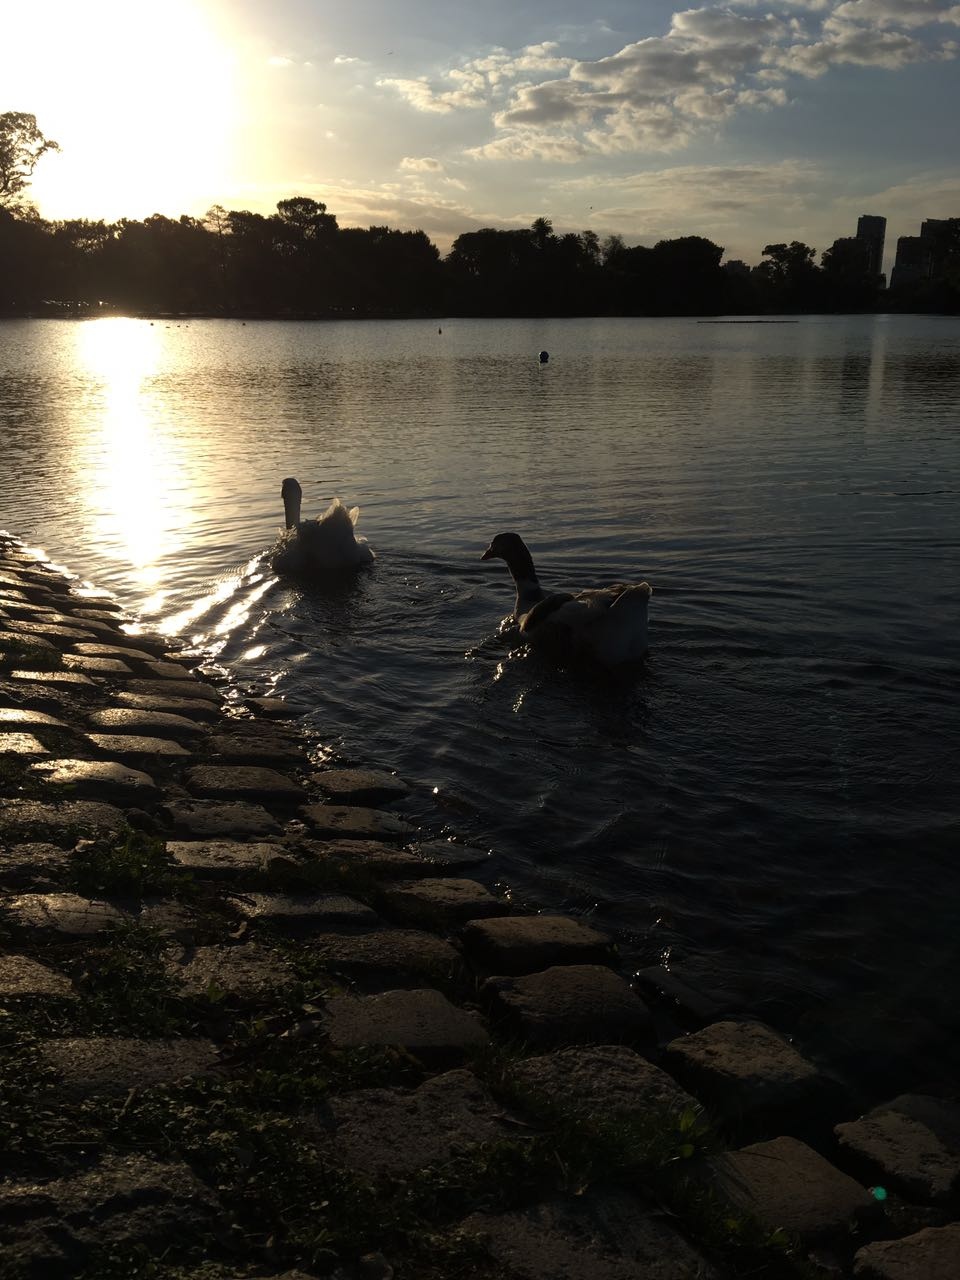
\includegraphics[width=0.3\textwidth]{patitos1.jpg}
        \caption{Imagen original}
\end{figure}

\begin{figure}[H]	
	\centering
    \begin{subfigure}{0.3\textwidth}
        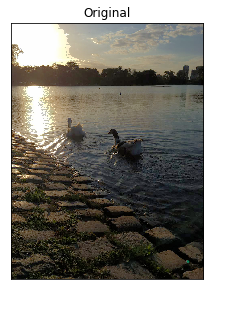
\includegraphics[width=0.9\textwidth]{patitos-k2.png}
        \subcaption{$k=2$}
    \end{subfigure}\hfill
    	\centering
    \begin{subfigure}{0.3\textwidth}
        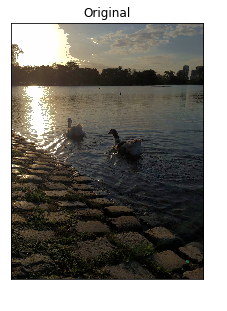
\includegraphics[width=0.9\textwidth]{patitos-k4.png}
        \subcaption{$k=4$}
    \end{subfigure}\hfill	
    \centering
    \begin{subfigure}{0.3\textwidth}
        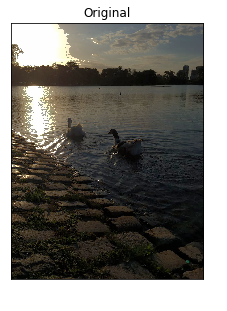
\includegraphics[width=0.9\textwidth]{patitos-k16.png}
        \subcaption{$k=16$}
    \end{subfigure}\hfill
\end{figure}

Al comparar las imágenes, se puede observar que a medida que se aumenta el $K$, la imagen se iba oscureciendo cada vez más. Debido a esto, nos fijamos que el valor de $alpha$ seleccionado automáticamente en el último subhistograma era de 1.0 (no variando estos valores) y el valor de $\beta$ del primer subhistrograma era de aproximadamente $0.998$ (ecualizando mucho los valores oscuros). Estos fueron los histogramas ecualizados finales de cada imagen:

\begin{figure}[H]
	\centering
        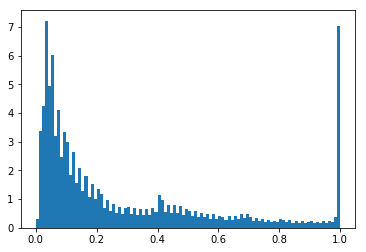
\includegraphics[width=0.3\textwidth]{patitos1-histogramaOriginal.png}
        \caption{Histograma de imagen original}
\end{figure}

\begin{figure}[H]	
	\centering
    \begin{subfigure}{0.3\textwidth}
        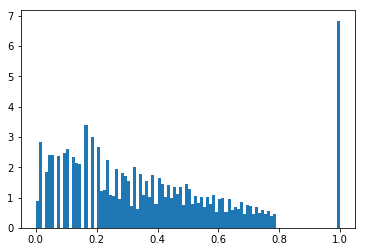
\includegraphics[width=0.9\textwidth]{patitos-histogramaFinal-k2.png}
        \subcaption{Histograma ecualizado con $k=2$}
    \end{subfigure}\hfill
    	\centering
    \begin{subfigure}{0.3\textwidth}
        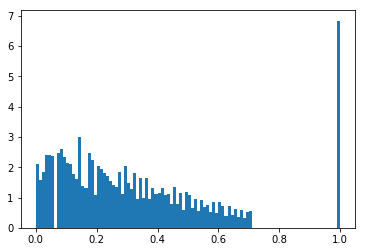
\includegraphics[width=0.9\textwidth]{patitos-histogramaFinal-k4.png}
        \subcaption{Histograma ecualizado con $k=4$}
    \end{subfigure}\hfill	
    \centering
    \begin{subfigure}{0.3\textwidth}
        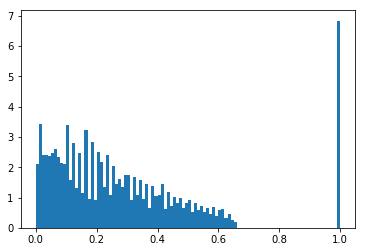
\includegraphics[width=0.9\textwidth]{patitos-histogramaFinal-k16.png}
        \subcaption{Histograma ecualizado con $k=16$}
    \end{subfigure}\hfill
\end{figure}

Así pudimos ver que en el caso de estas imágenes que poseen muchos píxeles claros, a medida que se va aumentando el valor de $k$, los histogramas tienden a ir concentrándose hacia valores de gris oscuros, en vez de generarse una ecualización equilibrada sobre todos los valores, ya que mantiene en el histograma final la cantidad elevada de valores de $gris=255$ y ecualiza los oscuros. Resultados similares fueron obtenidos con diversas imágenes con características similares. 

\subsubsection{Experimento 2}

Realizamos otros experimentos tomando imágenes provistas por la cátedra, cuya característica es que en su mayoría son oscuras, fijamos los parámetros $\alpha$ y $\beta$, y fuimos variando los valores de $k$. Obtuvimos los siguientes resultados:

\begin{figure}[H]
	\centering
        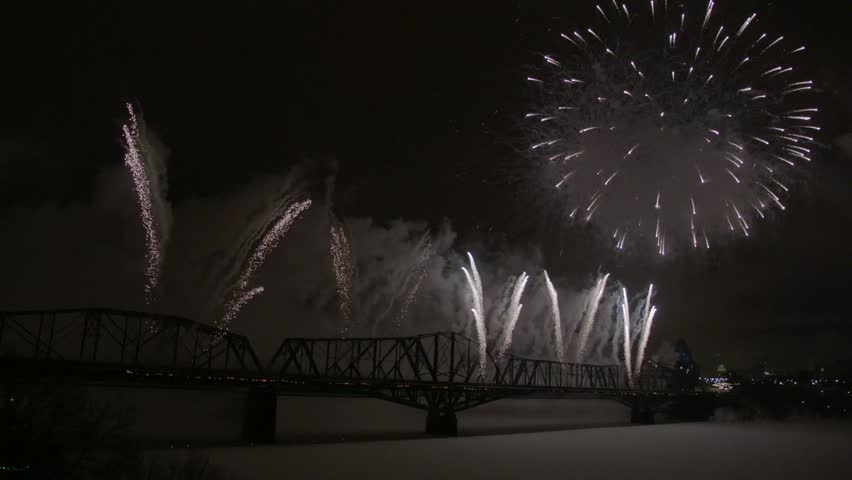
\includegraphics[width=0.3\textwidth]{fireworks.jpg}
        \caption{Imagen original}
\end{figure}

\begin{figure}[H]	
	\centering
    \begin{subfigure}{0.3\textwidth}
        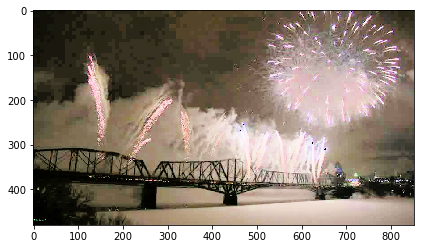
\includegraphics[width=0.9\textwidth]{fireworks-k4.png}
        \subcaption{$k=4$}
    \end{subfigure}\hfill
    	\centering
    \begin{subfigure}{0.3\textwidth}
        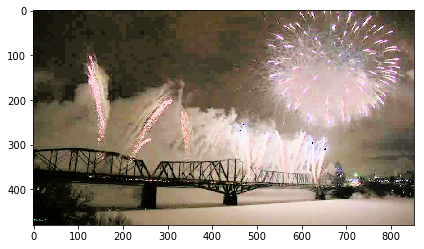
\includegraphics[width=0.9\textwidth]{fireworks-k8.png}
        \subcaption{$k=8$}
    \end{subfigure}\hfill	
    \centering
    \begin{subfigure}{0.3\textwidth}
        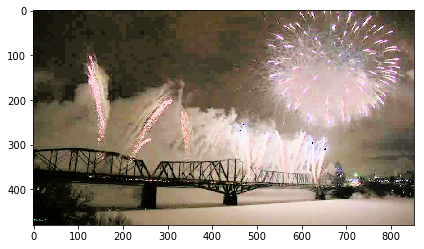
\includegraphics[width=0.9\textwidth]{fireworks-k16.png}
        \subcaption{$k=16$}
    \end{subfigure}\hfill
\end{figure}

\begin{figure}[H]
	\centering
        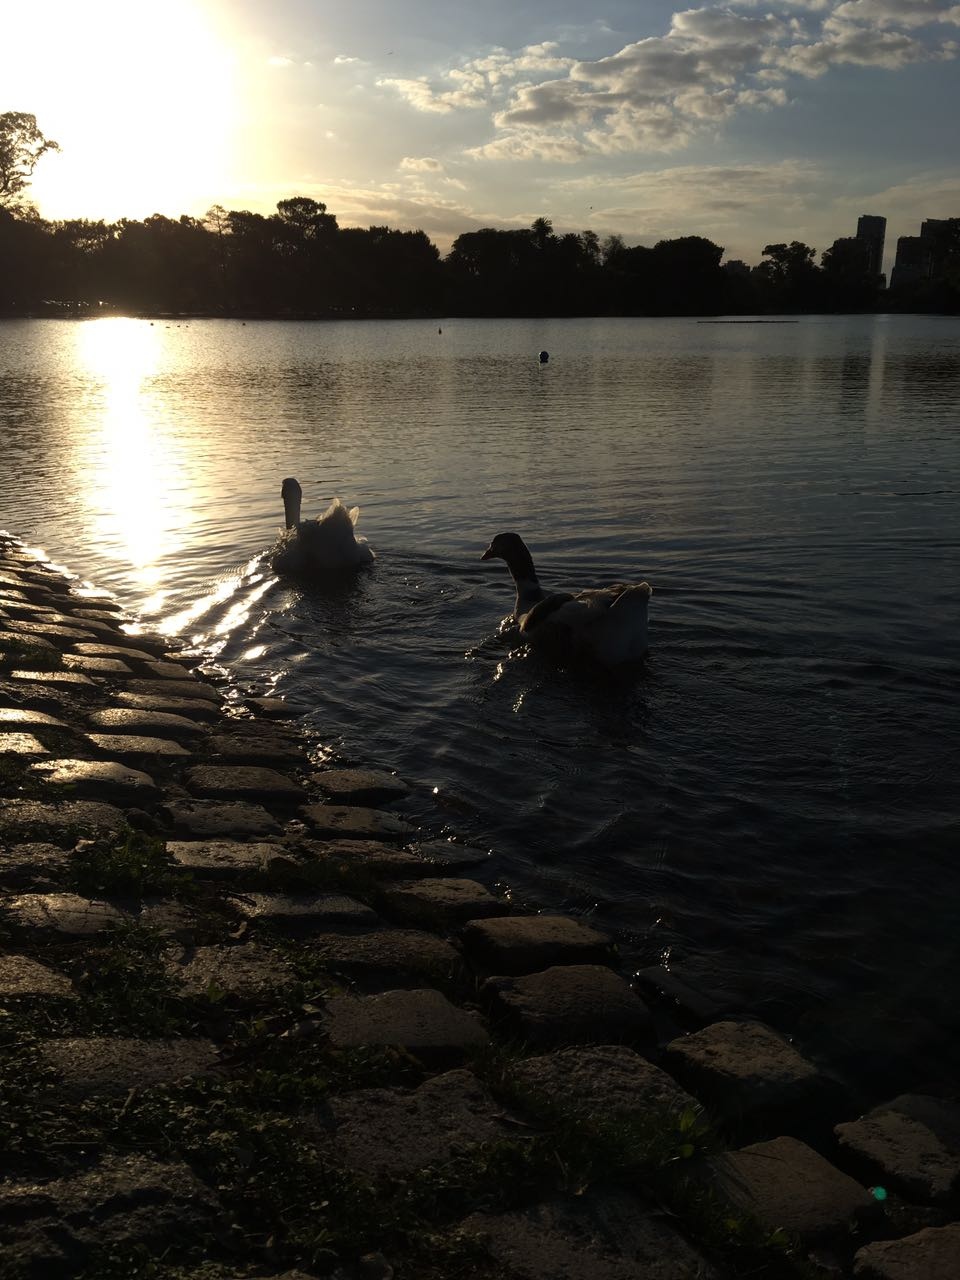
\includegraphics[width=0.3\textwidth]{patitos1.jpg}
        \caption{Imagen original}
\end{figure}

\begin{figure}[H]	
	\centering
    \begin{subfigure}{0.3\textwidth}
        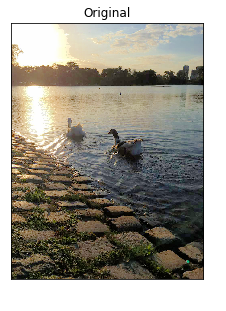
\includegraphics[width=0.9\textwidth]{patitos-alphabetafijos-k4.png}
        \subcaption{$k=4$}
    \end{subfigure}\hfill
    	\centering
    \begin{subfigure}{0.3\textwidth}
        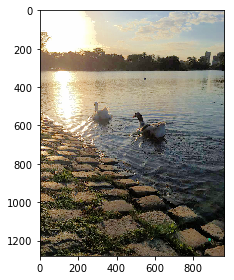
\includegraphics[width=0.9\textwidth]{patitos-alphabetafijos-k8.png}
        \subcaption{$k=8$}
    \end{subfigure}\hfill	
    \centering
    \begin{subfigure}{0.3\textwidth}
        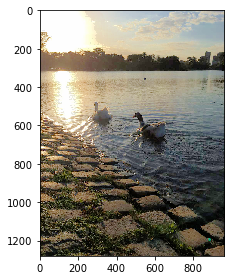
\includegraphics[width=0.9\textwidth]{patitos-alphabetafijos-k16.png}
        \subcaption{$k=16$}
    \end{subfigure}\hfill
\end{figure}


Si bien se puede observar un muy leve cambio entre las imágenes con $k=4$ y las demás, pudimos ver que a medida que se va aumentando el valor de $k$ para $k \geq 4$ no se producían cambios muy significativos y que el tiempo de cómputo aumentaba, por lo cual el valor de éste parámetro puede dejarse fijo en $k=3$ por ejemplo, como lo propone el paper.

\newpage 

\begin{thebibliography}{9}
\bibitem{paper}
Zhigang Ling, Yan Liang, Yaonan Wang, He Shen, Xiao Lu. \textit{Adaptive extended piecewise histogram equalisation for dark image enhancement.} IET Image Processing. 2015.
\end{thebibliography}


\end{document}